\begin{SCn}
\bigskip
\scnsectionheader{\currentname}

\scnstartsubstruct

\scnheader{Предметная область и онтология методов и средств реализации целенаправленного и персонифицированного процесса обучения пользователей для каждой ostis-системы, входящей в состав Экосистемы OSTIS}
\scnsdmainclasssingle{***}
\scnsdclass{***}
\scnsdrelation{***}

\scnheader{обучаемость}
\scnidtf{способность системы приобретать новые знания и навыки}
\scnrelfrom{включение}{неограниченная обучаемость}

\scnheader{неограниченная обучаемость}
\scnidtf{степень обучаемости, при которой не
накладывается никаких ограничений на типологию приобретенных знаний и навыков}
\scnexplanation{Говоря другими словами, система,
обладающая неограниченной обучаемостью, при необходимости может с течением времени приобрести любое знание и способность решать любую задачу}
	\scnaddlevel{1}
	\scnnote{Уточним, что это не означает, что одна конкретная система будет уметь решать любую задачу, это означает, что система может приобрести способность решать нужную ей задачу, при этом нет принципиальных ограничений на класс таких задач.}
	\scnaddlevel{-1}
	
\scnheader{интеллектуальная компьютерная система}
\scnidtf{сложная техническая система, разработка и даже использование которой требует высоких профессиональных качеств}
\scnrelfromset{проблемы текущего состояния}{\scnfileitem{недостаточная эффективность использования современных интеллектуальных систем, трудоемкость их внедрения и сопровождения, которые в значительной мере определяются высоким порогом вхождения конечных пользователей в интеллектуальные системы}
;\scnfileitem{пользователь часто не использует значительную часть функций даже традиционных компьютерных
систем просто по той причине, что не знает об их наличии и не имеет простого механизма, позволяющего о них узнать. Для интеллектуальных систем данная проблема стоит еще более остро}
;\scnfileitem{высоки затраты на обучение разработчиков интеллектуальных систем, на их адаптацию под особенности устройства конкретной интеллектуальной системы}}
	\scnaddlevel{1}
	\scnnote{Перечисленные трудности связаны не только с естественной сложностью интеллектуальных компьютерных
систем по сравнению с традиционными компьютерными системами, но с низким уровнем документации
для таких систем, неудобством использования такой
документации, трудоемкостью локализации средств
и области решения той или иной задачи, как для
конечного пользователя, так и для разработчика.}
	\scnaddlevel{-1}
\scnrelfrom{предлагаемый подход}{Подход к решению проблемы обучения конечных пользователей и разработчиков интеллектуальных систем}

\scnheader{Подход к решению проблемы обучения конечных пользователей и разработчиков интеллектуальных систем}
\scnidtf{подход к решению указанных проблем, предполагающий дополнение каждой интеллектуальной системы модулем, представляющим собой интеллектуальную обучающую подсистему}
	\scnaddlevel{1}
	\scnnote{Целью данной подсистемы является обучение конечного пользователя и разработчика основной системы принципам работы с ней, принципам ее функционирования и развития.}
	\scnaddlevel{-1}
\scntext{основная идея}{Независимо от того, для решения каких задач разрабатывается интеллектуальная система, она должна обладать некоторыми функциями обучающей системы, даже если система изначально не является обучающей.}
	\scnaddlevel{1}
	\scnexplanation{Следовательно,
	\begin{scnitemize}
	\item пользователь должен иметь возможность
обучаться как принципам работы с интеллектуальной системой, так и иметь возможность получать
новые знания о той предметной области, для которой создается интеллектуальная система;
	\item разработчик интеллектуальных систем должен иметь возможность обучаться принципам внутреннего устройства системы, принципам ее функционирования,
назначению конкретных компонентов системы, иметь возможность локализовать ту часть системы, в которой он должен разобраться для внесения изменений в функциональные возможности системы.	
	\end{scnitemize}}
	\scnnote{Для реализации данной идеи интеллектуальная система должна содержать не только знания о той предметной области, для которой она разработана, но и:
\begin{scnitemize}
\item знания о самой себе, своей архитектуре, компонентах, функциях, принципах работы и т.д.;
\item знания о пользователе, его опыте, навыках, предпочтениях, интересах;
\item знания о задачах, которые решает сама система в
текущий момент и задачах которые планируются к решению в будущем;
\item знания об актуальных задачах по развитию системы и ее сопровождению. 
\end{scnitemize}}
	\scnaddlevel{-1}
\scnrelfrom{технологическая основа}{модель представления знаний в виде унифицированных семантических сетей с теоретико-множественной интерпретацией}
	\scnaddlevel{1}
	\scnrelfromset{возможности}{
	\scnfileitem{Указанная модель является универсальной, то есть позволяет представлять в виде однородных семантических сетей знания любого рода, в том числе конкретные факты, логические утверждения (аксиомы, теоремы, определения), текстовые и мультимедийные иллюстрации и комментарии, примеры конкретных задач с решениями, в том числе доказательства и т.д.}
	;\scnfileitem{Подобная модель представления знаний позволяет рассматривать базу знаний любой системы как иерархию предметных областей, то есть позволяет произвести семантическую структуризацию предлагаемого учащемуся материала, что существенно облегчает процесс обучения за счет систематизации знаний на основе именно их семантики, а не каких-либо других сторонних факторов. Кроме этого, знания в базе могут делиться на логические разделы, каждый из которых соответствует какому-либо фрагменту излагаемого материала. Представление знаний в виде семантической сети позволяет осуществлять свободную навигацию по любым ассоциативным связям, изучая таким образом материал в той последовательности, какая кажется более логичной для самого обучаемого. С другой стороны, такой подход позволяет указать рекомендуемую последовательность изучения материала. При необходимости структура предметных областей может быть легко перестроена.}
	;\scnfileitem{Модель представления является унифицированной, то есть знания из различных областей представляются в сходном виде, что позволяет говорить не о семействе не связанных между собой обучающих систем по различным предметным областям, а о глобальном смысловом пространстве, объединяющем в себе знания всего семейства разрабатываемых систем. В свою очередь, наличие такого смыслового пространства обеспечивает ряд дополнительных возможностей:
	\begin{scnitemize}
	\item каждая система при необходимости может использовать знания, относящиеся к другим системам, что позволяется задавать не только вопросы, касающиеся конкретной предметной области, но и вопросы, носящие междисциплинарный характер;
	\item в рамках глобального смыслового пространства можно выделить часть знаний, которые имеют отношение ко многим системам из всего комплекса, например базовые знания из области математики, логики и т.д. Концепция глобального смыслового пространства позволяет записывать такие фрагменты знаний только в одной из систем, а затем использовать их во всех остальных, что существенно уменьшает количество дублирований, сокращает сроки разработки систем и снижает накладные расходы.
	\end{scnitemize}}
	;\scnfileitem{Рассматриваемый подход к представлению знаний позволяет унифицировать не только модель представления знаний, но и модели обработки знаний, в том числе модели информационного поиска и решения задач. Данный факт позволяется говорить о возможности реализации универсального набора поисковых операций, а также о реализации универсального решателя задач, позволяющего решать различные задачи в рамках каждой из рассматриваемых предметных областей, что существенно сокращает количество реализуемых операций обработки знаний при сохранении функциональных возможностей каждой системы.}
	;\scnfileitem{Как уже было сказано выше, унифицированная модель представления знаний позволяет не только вносить в каждую систему примеры условий типовых для заданной предметной области задач с решениями, но и говорить об интеллектуальном решателе, который позволит системе генерировать ответы на поставленный вопрос за счет знаний уже имеющихся в базе знаний, например с использованием правил логического вывода.}
	;\scnfileitem{Унифицированное представление знаний позволяет не ограничивать номенклатуру пользовательских запросов только специально выделенными для этого командами, а задавать произвольный запрос системе с использованием универсального языка отображения знаний, что делает перечень возможных запросов зависящим только от количества и разнообразия знаний, внесенных в базу знаний системы.}
	;\scnfileitem{Унификация моделей пользовательских интерфейсов позволяет отображать знания различного рода в унифицированном виде независимо от предметной области, к которой эти знания относятся. Таким образом, все разрабатываемые системы будут обладать пользовательским интерфейсом, построенным по одним и тем же принципам, что позволит существенно сократить срок ознакомления учащегося со всем семейством систем. Данный факт не отрицает возможность и необходимость разработки отдельных компонентов интерфейса, ориентированных на конкретную предметную область, например, редактора геометрических чертежей, виртуальной лаборатории для проведения химических опытов и т.д.}
	;\scnfileitem{Каждый компонент пользовательского интерфейса также является отображением определенного элемента из базы знаний, что позволяет, во-первых, легко менять интерфейс системы даже во время ее работы, а, во-вторых, позволяет пользователю задавать системе вопросы не только касательно предметной области, которой посвящена данная система, но и касательно любого из компонентов интерфейса и других частей системы. Таким образом, пользователю достаточно научиться задавать системе несколько простейших вопросов, чтобы в дальнейшем изучить все тонкости работы системой уже в процессе общения с ней.}
	;\scnfileitem{Предлагаемые модели представления и обработки знаний позволяют физически отделить смысл хранимой информации от вариантов ее внешнего отображения, в частности, от идентификаторов тех или иных сущностей в рамках какого-либо естественного языка. Это дает возможность легко интернационализировать любую из разработанных систем, поскольку для перевода системы на какой-либо другой язык необходимо перевести только фрагменты текстов на естественном языке, явно хранимые в базе знаний, не затрагивая при этом сами семантические связи, то есть смысл представленной информации.}}
	\scnaddlevel{-1}
\scnrelfrom{модель обработки знаний}{модель, основанная на многоагентном подходе}
	\scnaddlevel{1}
	\scnrelfromset{преимущества}{
	\scnfileitem{Работа агентов осуществляется независимо друг от друга, что позволяет легко расширять функционал той или иной системы при необходимости, а также позволяет интегрировать в одной и той системе различные модели информационного поиска, решения задач и т.д.}
	;\scnfileitem{Работа агентов осуществляется параллельно, что существенно улучшает производительность всей системы в целом.}}
	\scnaddlevel{-1}
\scnrelfrom{предлагаемый фундамент}{\scnkeyword{Технология OSTIS}}
	\scnaddlevel{1}
	\scnidtf{открытая семантическая технология проектирования интеллектуальных систем}
	\scnnote{\textit{Технология OSTIS} позволяет интегрировать любые виды знаний и любые модели решения задач}
	\scnrelfromset{преимущества}{
\scnfileitem{В основе технологии лежит \textit{SC-код} -- универсальный и унифицированный язык кодирования информации в графодинамической памяти компьютерных систем. \textit{SC-код} позволяет в унифицированном (одинаковом) виде представить любую информацию, что позволит сделать предлагаемый подход универсальным и подходящим для любого класса интеллектуальных систем}
;\scnfileitem{\textit{Технология OSTIS} и, в частности, \textit{SC-код}, легко интегрируется с любыми современными технологиями, что позволит применить предлагаемый подход для большого числа уже разработанных интеллектуальных систем}
;\scnfileitem{\textit{SC-код} позволяет хранить и описывать в базе знаний ostis-системы любую внешнюю (инородную)
по отношению к \textit{SC-коду} информацию в виде внутренних файлов \textit{ostis-систем}. Таким образом, база знаний обучающей подсистемы может содержать в явном виде фрагменты уже имеющейся документации к системе, представленной в любой форме}
;\scnfileitem{В рамках \textit{Технологии OSTIS} уже разработаны модели баз знаний \textit{ostis-систем}, решателей задач \textit{ostis-систем} и пользовательских интерфейсов \textit{ostis-систем}, предполагающие полное их описание в базе знаний системы. Таким образом для \textit{ostis-систем} предлагаемый подход реализуется значительно проще и дает дополнительные преимущества, подробнее рассмотренные
в работе}
;\scnfileitem{одним из основных принципов \textit{Технологии OSTIS} является обеспечение гибкости (модифицируемости) систем, разрабатываемых на ее основе. Таким образом, использование \textit{Технологии OSTIS} обеспечит возможность эволюции самой интеллектуальной обучающей подсистемы}}
	\scnaddlevel{-1}

\scnheader{интеллектуальная обучающая система}
\scnsuperset{интеллектуальная система}
\scnnote{Такого рода системы по сравнению с традиционными системами электронного обучения (например, электронными учебниками) предоставляют обладают рядом существенных преимуществ.}
\scnnote{В случае реализации \textit{интеллектуальной обучающей системы} на основе \textit{Технологии OSTIS}, появляются дополнительные возможности, к числу которых можно отнести следующие:
	\begin{scnitemize}
	\item пользователю в явном виде представляется семантическая структура изучаемого учебного материала и изучаемой предметной области. При этом
обеспечивается наглядная визуализация любого
уровня указанной семантической структуры;
	\item пользователю становятся доступны достаточно полные сведения об изучаемой предметной области, отражены все ее аспекты, благодаря явному
помещению в базу знаний всех предметных закономерностей и взаимосвязей понятий;
	\item помимо возможности чтения текстов и иллюстративных материалов учебника предоставляется возможность навигации по семантическому пространству предметной области;
	\item пользователю предоставляется возможность задавать системе любые вопросы и задачи по изучаемой предметной области;
	\item пользователю предоставляется возможность под контролем системы тренироваться (приобретать практические навыки) в решении самых различных
задач по изучаемой предметной области.
 При этом система:
	\begin{scnitemizeii}
	\item осуществляет семантический анализ правильности решения задач как по свободно конструируемым ответам (результатам), так и по протоколам решения;
	\item локализует допущенные пользователем ошибки
в решении задач, определяет их причину и выдает соответствующие рекомендации пользователю.
	\end{scnitemizeii}
	\item при общении с системой пользователю предоставляется свобода в выборе любого из множества синонимичных терминов (идентификаторов), зарегистрированных в базе знаний системы;
	\item появляется принципиальная возможность реализации естественно-языкового интерфейса с пользователем (благодаря широким возможностям семантического анализа пользовательских сообщений и возможностям синтеза на семантическом уровне сообщений, адресуемых пользователям);
	\item пользователю предоставляется полная свобода в выборе последовательности изучения учебного материала (маршрута навигации по учебному материалу), в выборе решаемых им задач (в сборнике задач и лабораторных работ), но соответствующие рекомендации выдаются.
	\end{scnitemize}}
	\scnaddlevel{1}
	\scnnote{Часть из перечисленных возможностей (а в предельном случае и все их них) могут быть реализованы в рамках подсистемы обучения пользователей интеллектуальной системы.}
	\scnaddlevel{-1}


\scnheader{подсистема обучения пользователей интеллектуальных систем}
\scnexplanation{Для реализации взаимодействия \textit{подсистемы обучения пользователей интеллектуальных систем}, реализуемой на основе \textit{Технологии OSTIS} с основной \textit{интеллектуальной системой} предполагается разработка интерфейсного компонента, который также является частью подсистемы. Важно отметить, что для разных \textit{интеллектуальных систем} такие компоненты будут в значительной степени пересекаться, что, в свою очередь, позволит снизить затраты на интеграцию подсистемы обучения и основной \textit{интеллектуальной системы}}
\scnrelfrom{иллюстрация}{\scnfileimage{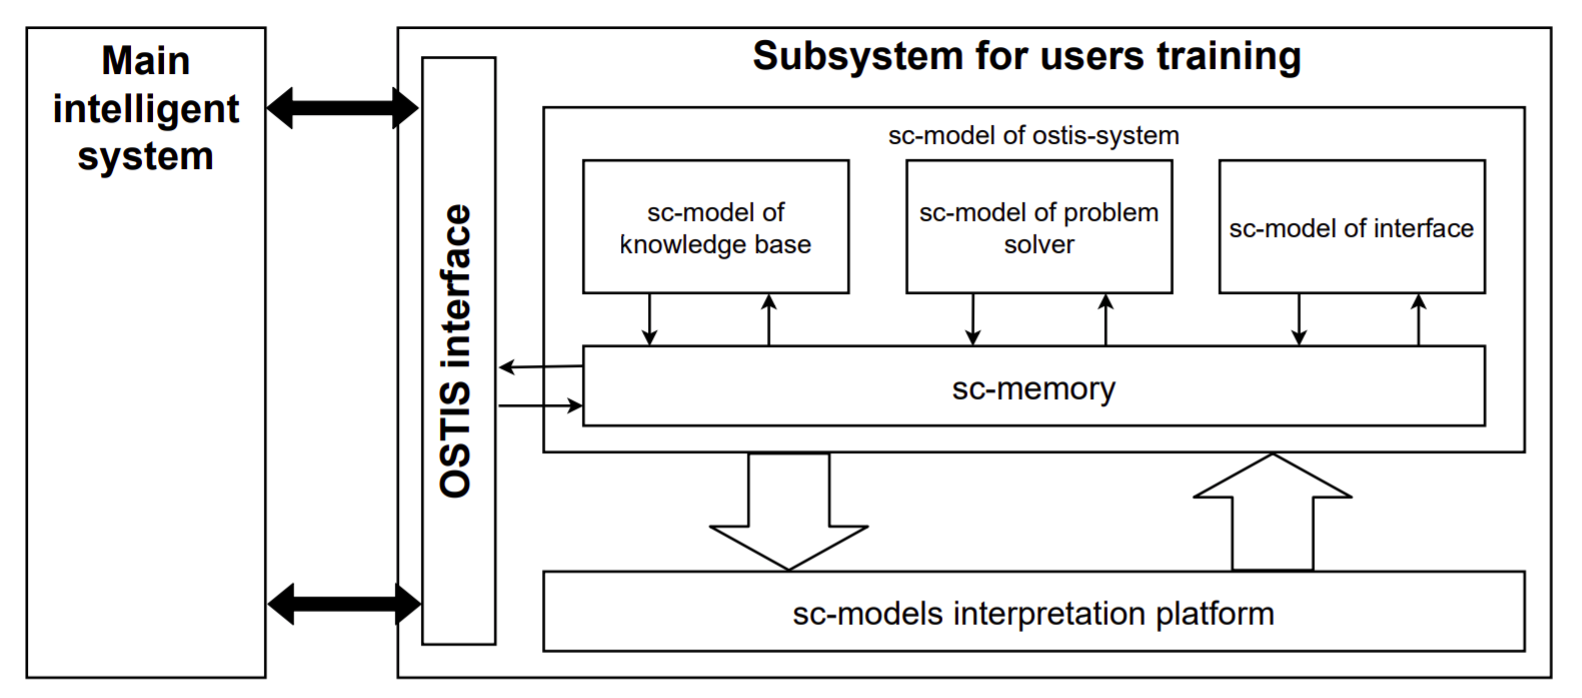
\includegraphics[width=0.7\linewidth]{figures/sd_learning/system_arch.png}}}

\scnnote{В случае, если рассматриваемая интеллектуальная система является \textit{ostis-системой}, ее интеграция с подсистемой обучения пользователей интеллектуальных систем осуществляется более глубоко и архитектуру полученной интегрированной системы можно изобразить следующим образом (см. Рис.\textit{ Архитектура подсистемы обучения пользователей интеллектуальных систем в составе другой ostis-системы}). Как видно из рисунка, компоненты \textit{подсистемы обучения пользователей интеллектуальных систем} просто дополняют уже существующие в основной ostis-системе компоненты, что позволяет максимально снизить затраты на интеграцию \textit{подсистемы обучения пользователей интеллектуальных систем} и основной \textit{ostis-системы}.}

\scnheader{Рис. Архитектура подсистемы обучения пользователей интеллектуальных систем в составе другой ostis-системы}
\scneqfile{\\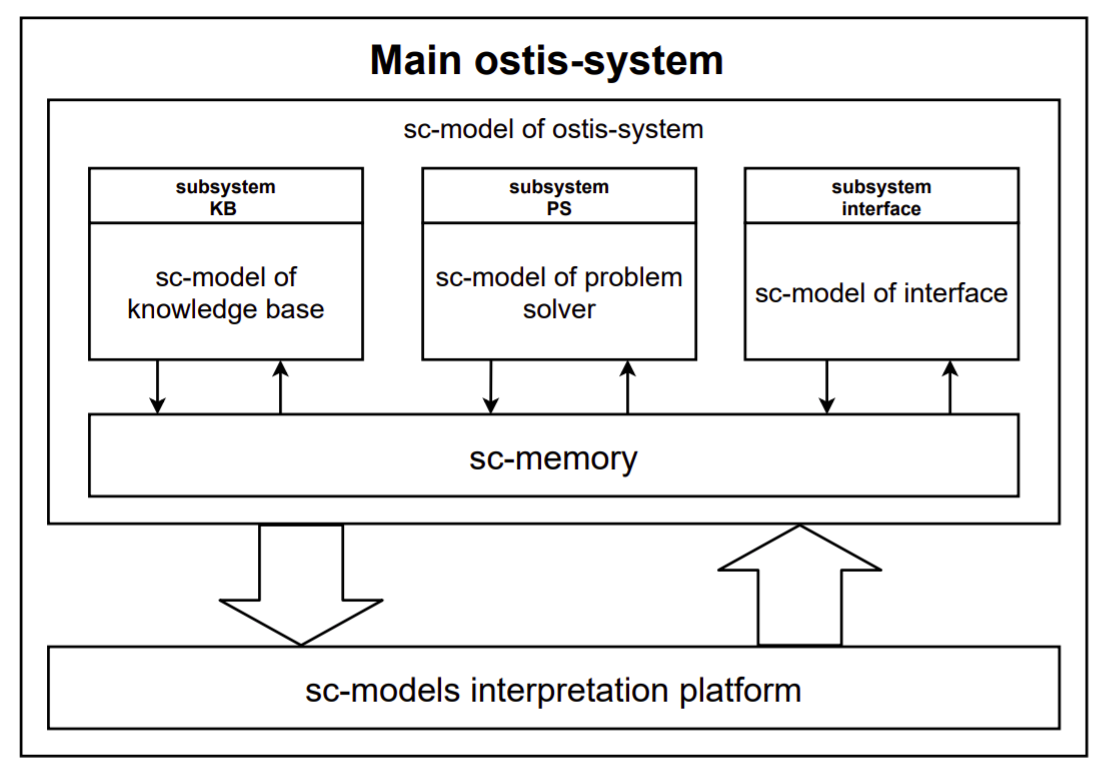
\includegraphics[width=0.5\linewidth]{figures/sd_learning/subsystem_arch.png}\\}

\scnheader{Подход к разработке баз знаний в подсистеме обучения пользователей интеллектуальных систем}

\scnrelfromlist{пример}{
\scnfileitem{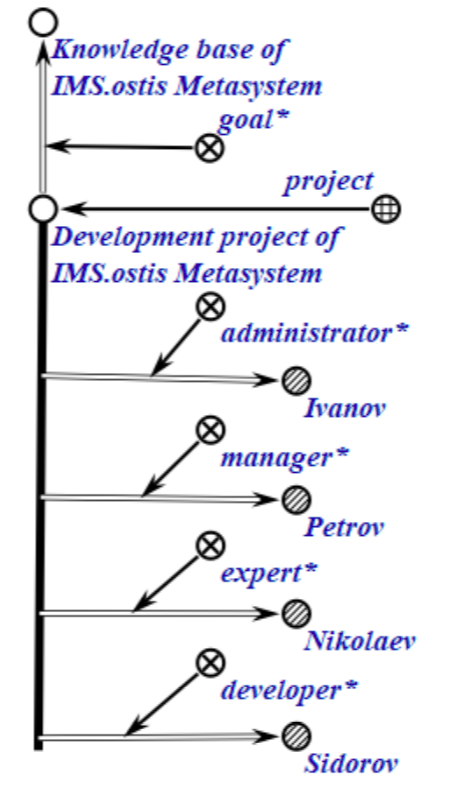
\includegraphics[width=0.3\linewidth]{figures/sd_learning/example_1.png}}
\scnaddlevel{1}
\scnnote{В данном примере показано, как используя средства структуризации баз знаний, разработанные в рамках Технологии OSTIS, можно описать в базе знаний различные виды информации об одной и той же сущности, в частности, текущую занятость и профессиональные навыки пользователя. Аналогичным образом можно описать любую другую информацию о пользователе.}
\scnaddlevel{-1};
\scnitem{
\scnaddlevel{1}
\textbf{\textit{семантическая модель базы знаний}}\\
\scnrelfromset{абстрактная базовая декомпозиция}{
история и текущие процессы эксплуатации компьютерной системы\\
	\scnrelfromset{абстрактная базовая декомпозиция}{
	\scnitem{история эксплуатации компьютерной системы}
	;\scnitem{текущие процессы эксплуатации компьютерной системы}}\\
;документация компьютерной системы
;контекст предметной части базы знаний в рамках Глобальной базы знаний
;предметная часть базы знаний
;история, текущие процессы и план развития компьютерной системы\\
	\scnrelfromset{абстрактная базовая декомпозиция}{
	\scnitem{текущие процессы развития компьютерной системы}
	;\scnitem{история развития компьютерной системы}
	;\scnitem{структура и организация проекта компьютерной системы}
	;\scnitem{план развития компьютерной системы}}}}
\scnnote{База знаний ostis-системы может быть структурирована по различным признакам. В данном примере наибольший интерес представляет структуризация базы знаний с точки зрения процесса ее разработки.}
\scnaddlevel{-1};
\scnfileitem{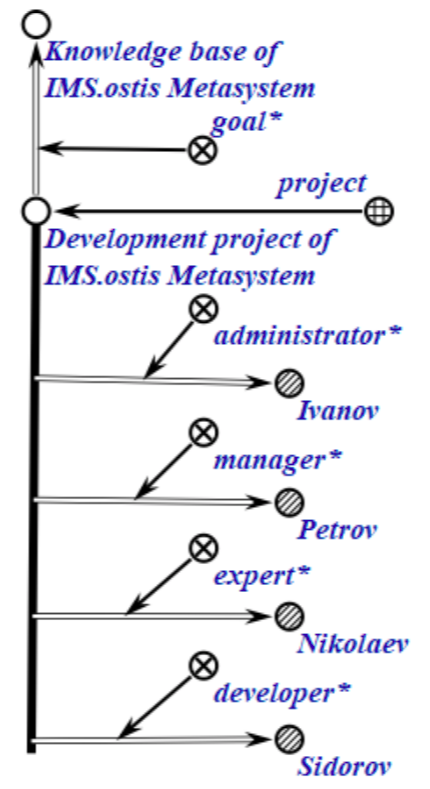
\includegraphics[width=0.3\linewidth]{figures/sd_learning/example_2.png}}
\scnaddlevel{1}
\scnnote{Выше показан пример описания информации об исполнителях некоторого проекта, выполняющих в нем различные роли. С точки зрения структуры базы знаний эта информация является частью раздела структура и организация проекта компьютерной системы.}
\scnaddlevel{-1};\scnfileitem{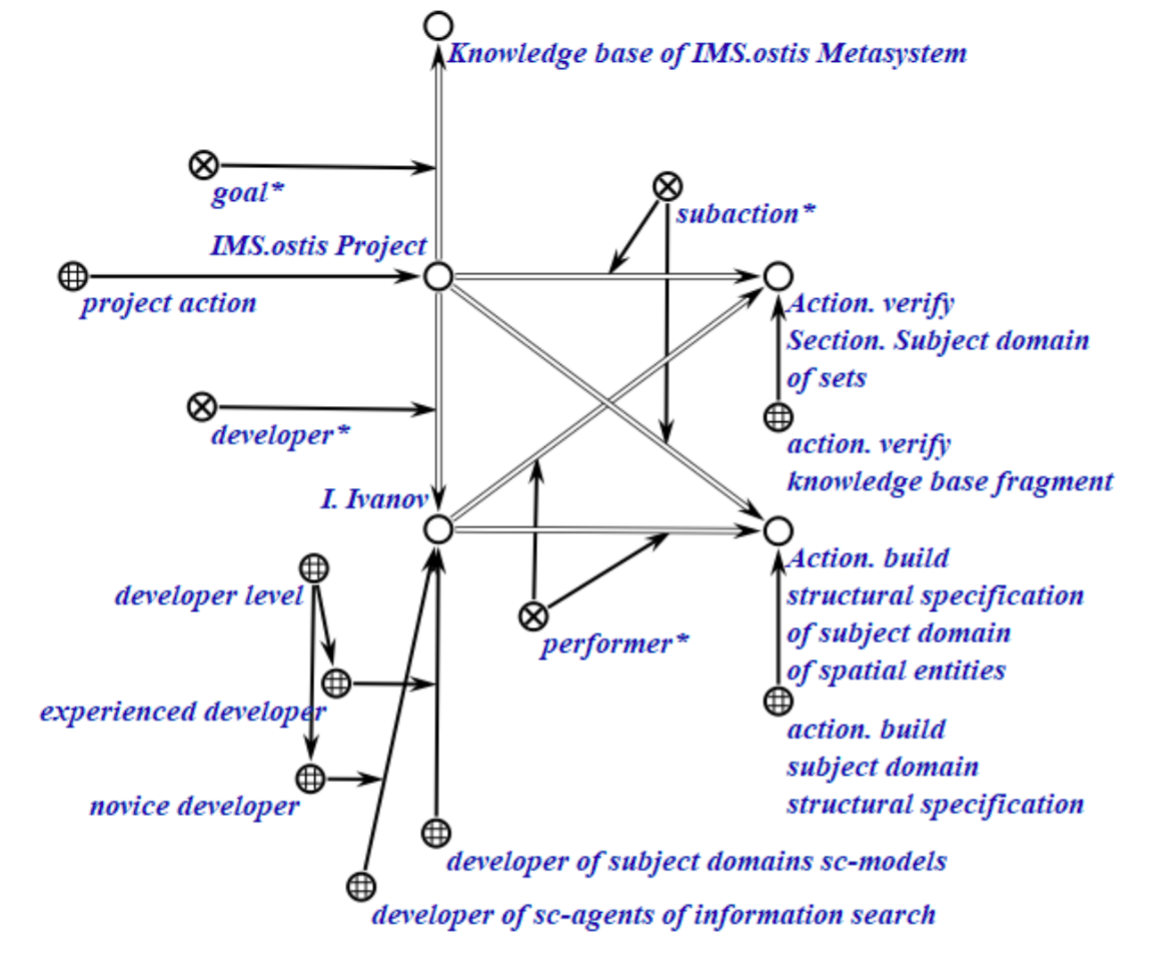
\includegraphics[width=0.6\linewidth]{figures/sd_learning/example_3.png}}
\scnaddlevel{1}
\scnnote{Выше показан пример описания проектных задач и их исполнителей с учетом квалификации каждого исполнителя. С точки зрения структуры базы знаний эта информация является частью раздела текущие процессы развития компьютерной системы.}
\scnaddlevel{-1};
\scnitem{
\scnaddlevel{1}
\textbf{\textit{Решатель задач системы контроля качества нанесения маркировки}}\\
\scnrelfromset{декомпозиция абстрактного sc-агента}{
Атомарный абстрактный sc-агент распознавания маркировки на основе нейронной сети
;Неатомарный абстрактный sc-агент принятия решений\\
	\scnrelfromset{декомпозиция абстрактного sc-агента}{
	Атомарный абстрактный sc-агент, реализующий концепцию пакета программ\\
	;Неатомарный абстрактный sc-агент достоверного вывода
	;Неатомарный абстрактный sc-агент правдоподобного вывода}\\
;Неатомарный абстрактный sc-агент ассоциативного поиска\\
;Неатомарный абстрактный sc-агент интерпретации программ управления роботизированной установкой\\
	\scnrelfromset{декомпозиция абстрактного sc-агента}{
	Атомарный абстрактный sc-агент интерпретации действия перемещения\\
	;Атомарный абстрактный sc-агент интерпретации действия захвата}}
\scnheader{Неатомарный абстрактный sc-агент достоверного вывода}
\scnrelfromset{декомпозиция абстрактного sc-агента}{
Атомарный абстрактный sc-агент, реализующий стратегию правдоподобного вывода\\
;Неатомарный абстрактный sc-агент интерпретации логических правил}
\scnheader{Неатомарный абстрактный sc-агент правдоподобного вывода}
\scnrelfromset{декомпозиция абстрактного sc-агента}{
Атомарный абстрактный sc-агент, реализующий стратегию правдоподобного вывода\\
;Неатомарный абстрактный sc-агент интерпретации логических правил}
\scnheader{Неатомарный абстрактный sc-агент интерпретации логических правил}
\scnrelfromset{декомпозиция абстрактного sc-агента}{
Атомарный абстрактный sc-агент применения импликативных правил\\
;Атомарный абстрактный sc-агент применения правил об эквиваленции}
}
\scnnote{Согласно предложенному в рамках Технологии OSTIS подходу к разработке решателей задач основу решателя составляет иерархическая система агентов над семантической памятью (sc-агентов). Структура решателя также может быть описана в базе знаний ostis-системе. В данном примере представлена структура решателя задач системы контроля качества нанесения маркировки для предприятия рецептурного производства}
\scnaddlevel{-1}}
\scnendstruct \scnendcurrentsectioncomment
\end{SCn}
